
\section{Datasets Overview}
Datasets considered by the validation procedure, already mentioned in the validation block diagram (Figure \ref{validation_strategy}).

\subsection{AIJ Dataset}
\url{https://www.aij.or.jp/jpn/publish/cfdguide/index_e.htm}\newline
% \begin{figure}[h!]
%     \centering
%     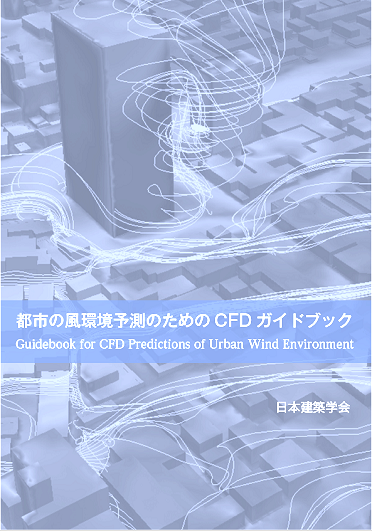
\includegraphics[scale=0.5]{imgs/aij_dataset_image.png}
%     \caption{For comparative analysis with respect to AIJ-A and AIJ-C}
% \end{figure}

\subsection{TPU Dataset}
\url{https://www.wind.arch.t-kougei.ac.jp/info_center/pollution/pollution.html}\newline
% \begin{figure}[h!]
%     \centering
%     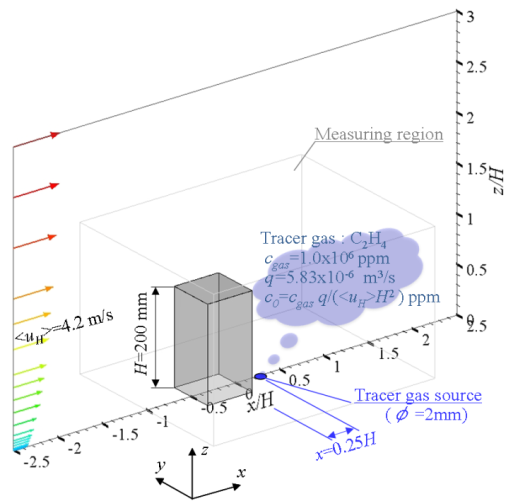
\includegraphics[scale=0.35]{imgs/tpu_dataset_image.png}
%     \caption{For comparative analysis TPU-A and TPU-B.} 
% \end{figure}

\subsection{StratEnFlo Dataset}
\url{https://figshare.com/articles/dataset/Array_of_buildings_with_incoming_stra-tification/8320007}\newline
% \vspace*{-0.2cm}\begin{figure}[h!]
%     \centering
%     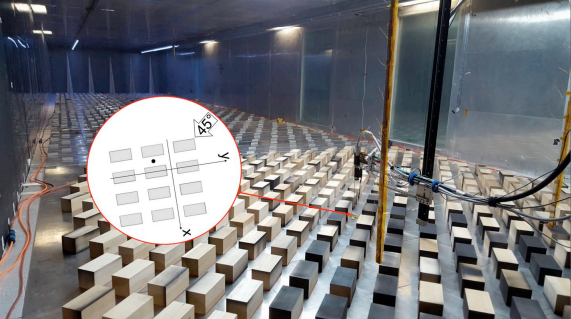
\includegraphics[scale=0.4]{imgs/sef_dataset_image.png}
%     \caption{For comparative analysis SEF-A, SEF-B, and SEF-C.} 
% \end{figure}

\subsection{COST ES 1006 Dataset}
\url{https://www.mi.uni-hamburg.de/en/arbeitsgruppen/windkanallabor/data-sets.html}\newline
% \begin{figure}[h!]
%     \centering
%     \begin{minipage}{0.38\textwidth}
%         \centering
%         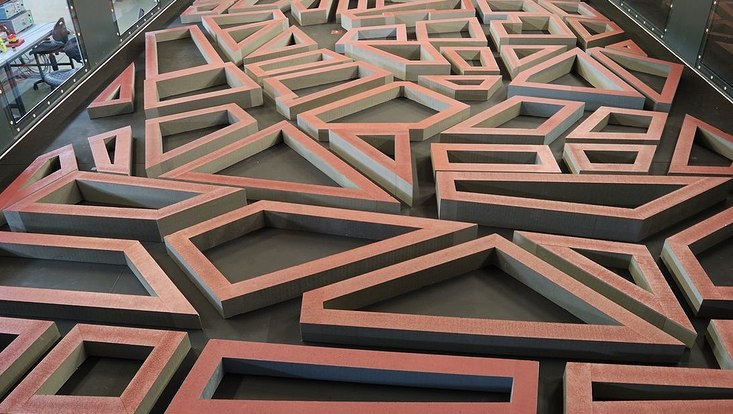
\includegraphics[width=\textwidth]{imgs/michelstad.jpg}
%         \caption{Michelstadt wind tunnel experiment (COST-M)}
%     \end{minipage}
%     \hfill
%     \begin{minipage}{0.38\textwidth}
%         \centering
%         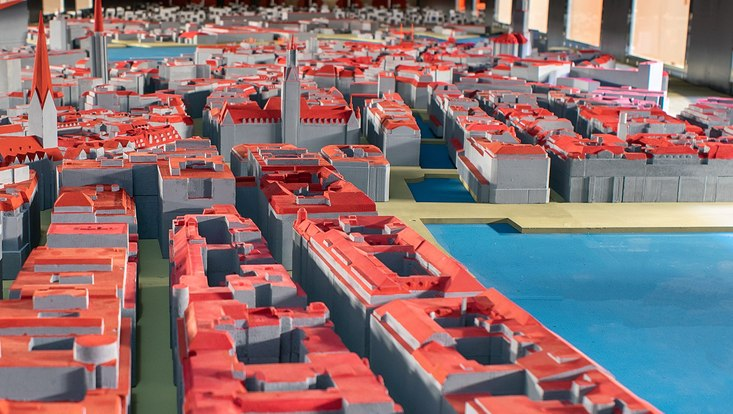
\includegraphics[width=\textwidth]{imgs/cute.jpg}
%         \caption{CUTE wind tunnel experiment (COST-C-WT) and its associated field experiment (COST-C-F).}
%     \end{minipage}
% \end{figure}

% \vspace*{-1cm}
\subsection{TURBAN Dataset}
\url{https://www.project-turban.eu/results_01_main.html}
% \vspace*{-0.2cm}\begin{figure}[h!]
%     \centering
%     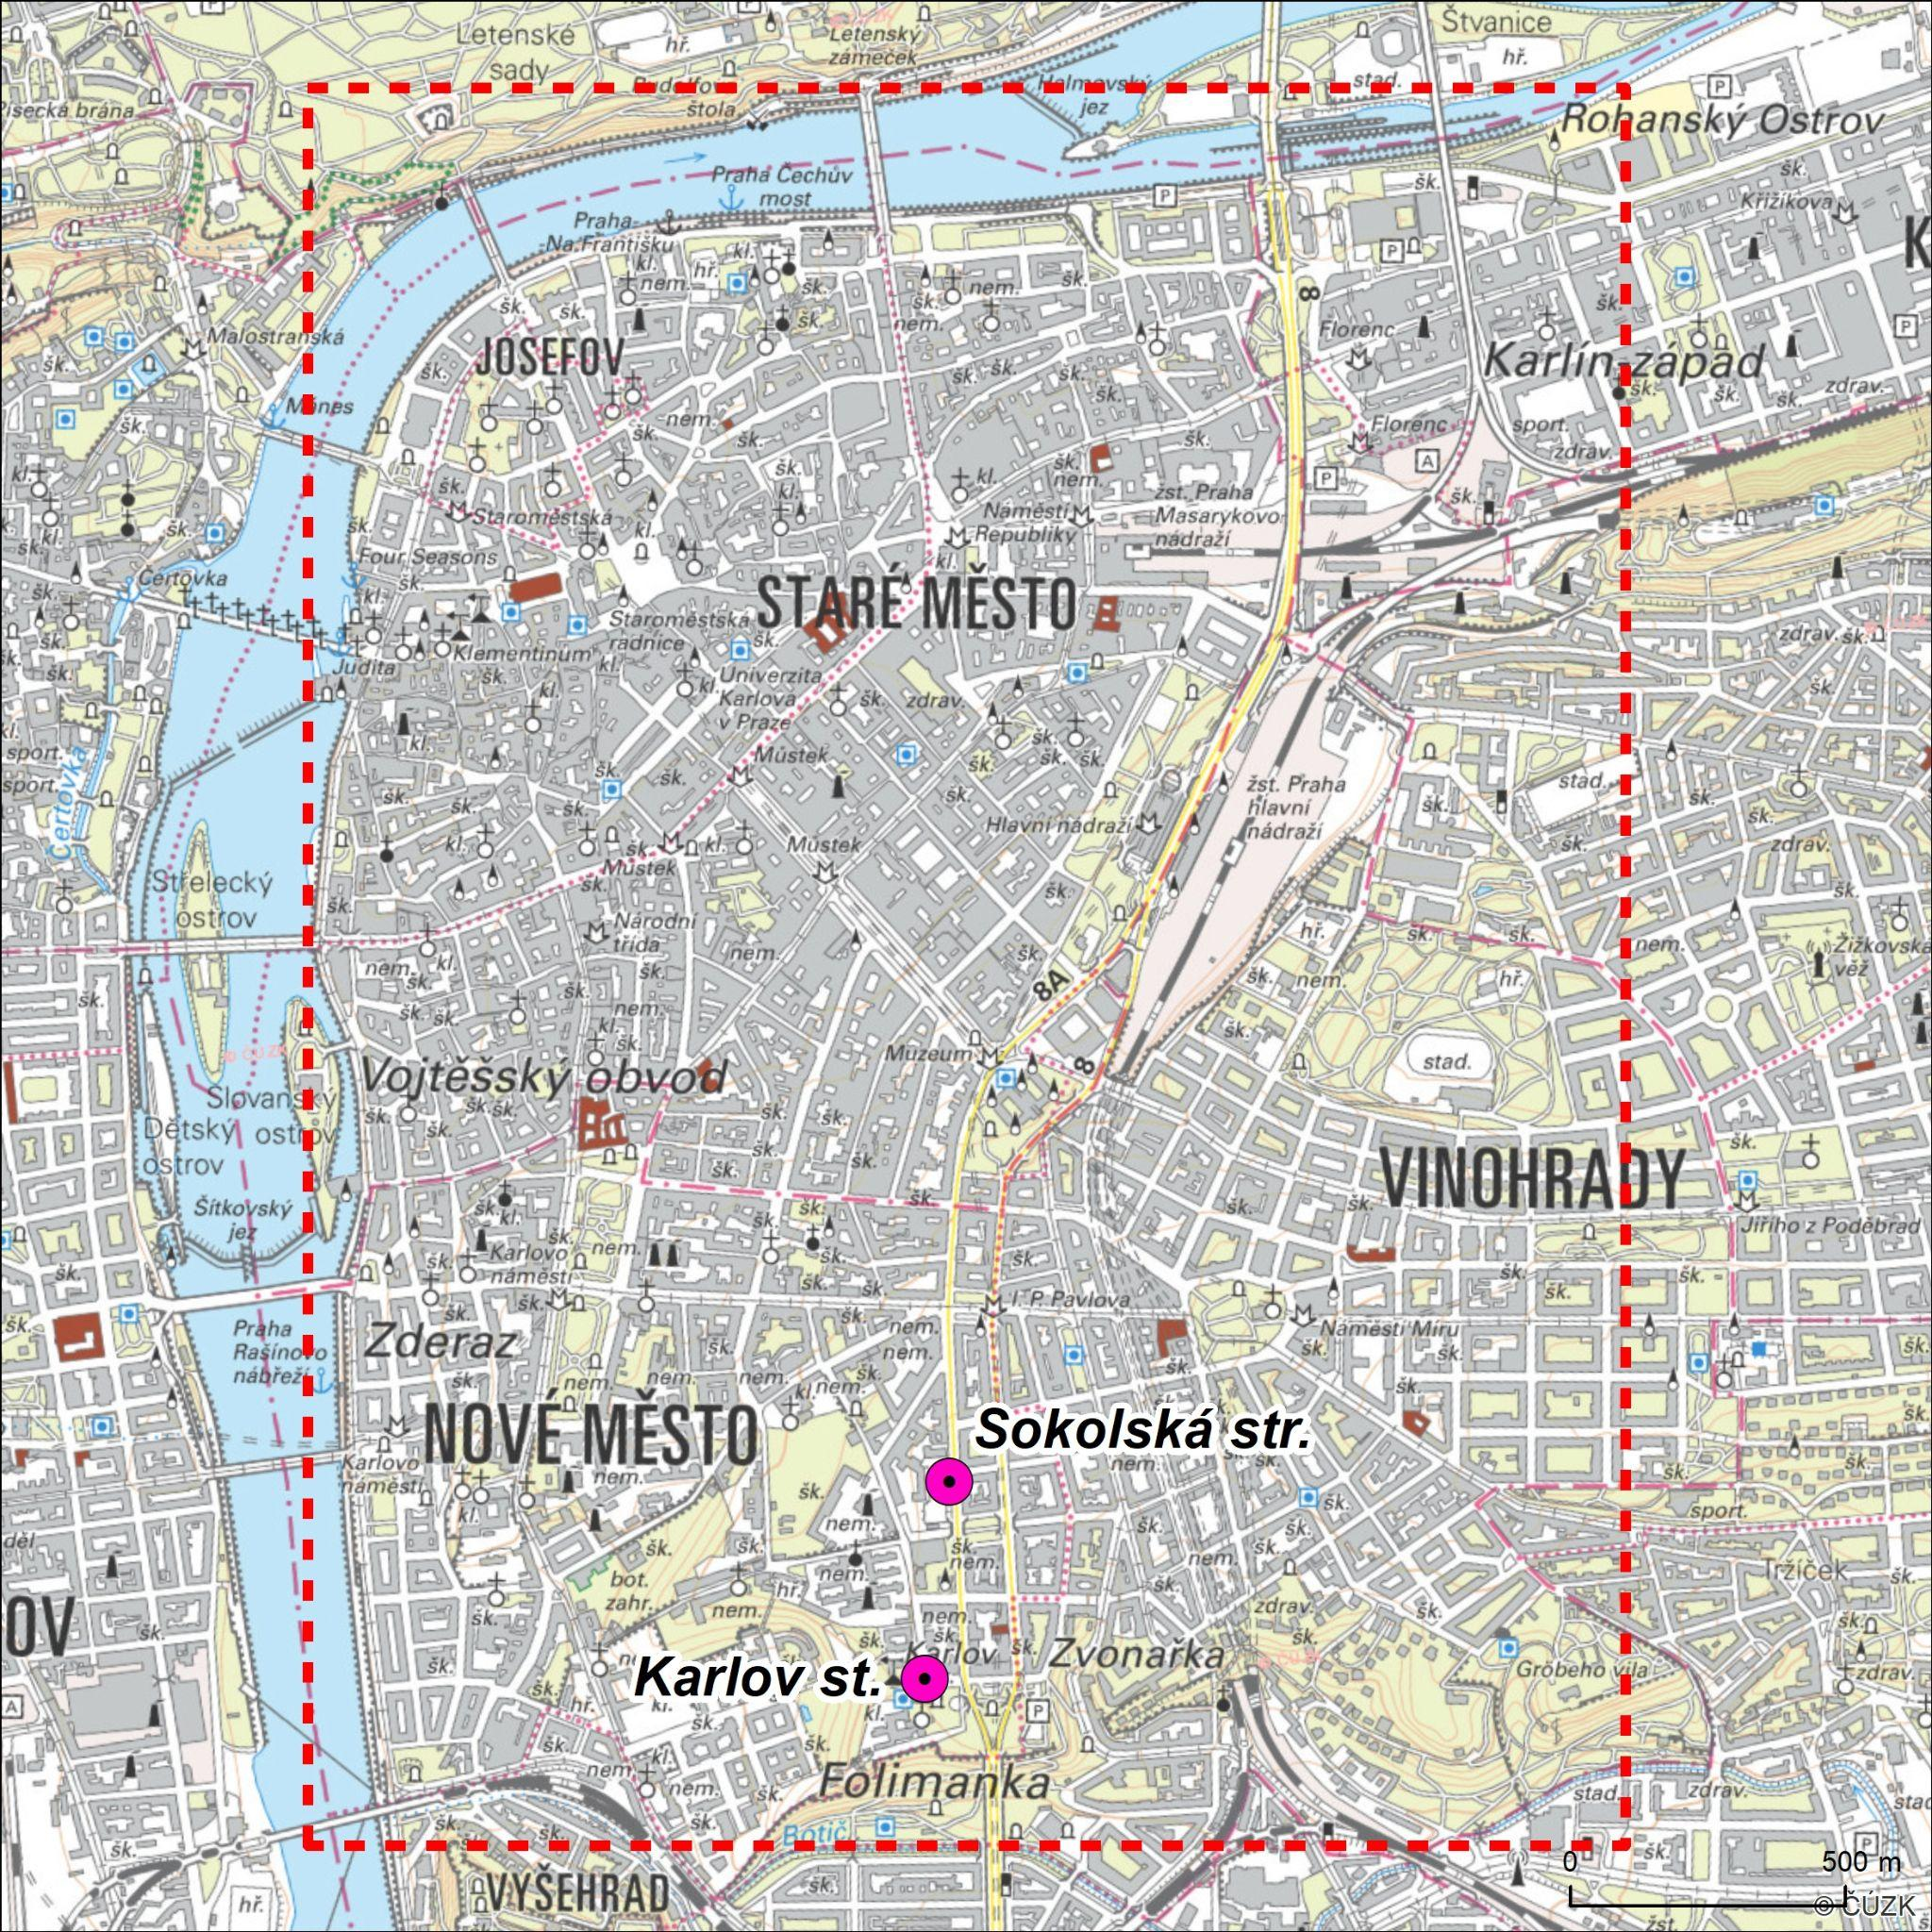
\includegraphics[scale=0.075]{imgs/turban_dataset_image.jpg}
%     \caption{Measurement campaign in the city of Prague (TURB-P)}
% \end{figure}

% \newpage


% \begin{enumerate}
%     \item \textbf{NSBL - Simple Obstacles:}
%     \begin{itemize}
%       \item[-] from AIJ Dataset: case A with single building, and case C with a street canyon (AIJ-A and AIJ-C).
%         \begin{figure}[h!]
%             \centering
%             \begin{minipage}{\dimexpr\textwidth-4cm}
%                 \begin{minipage}{0.45\textwidth}
%                     \centering
%                     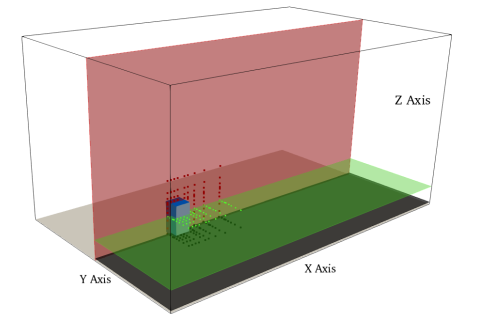
\includegraphics[width=\textwidth]{imgs/aij_A.png}
%                     \captionof{figure}{Single building in NSBL}
%                 \end{minipage}
%                 \hfill
%                 \begin{minipage}{0.45\textwidth}
%                     \centering
%                     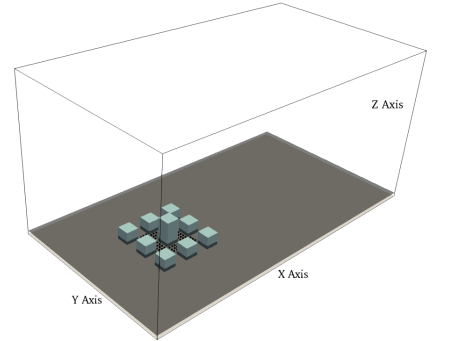
\includegraphics[width=\textwidth]{imgs/aij_C.png}
%                     \captionof{figure}{Street canyon in NSBL}
%                 \end{minipage}
%             \end{minipage}
%         \end{figure}
%         \item[-] from TPU Dataset: single building with dispersion of neutral substance (called \textit{isothermal case}, TPU-A).
%         \begin{figure}[h!]
%             \centering
%             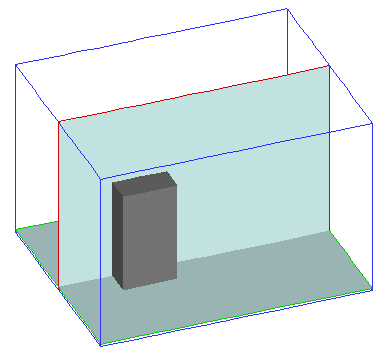
\includegraphics[width=0.35\textwidth]{imgs/tpu_1.png}
%         \end{figure}
%         \item[-] from StratEnFlo Dataset: street canyon with and without dispersion of heavy gas (NSBL configuration, SEF-B).
%             \begin{figure}[h!]
%               \centering
%               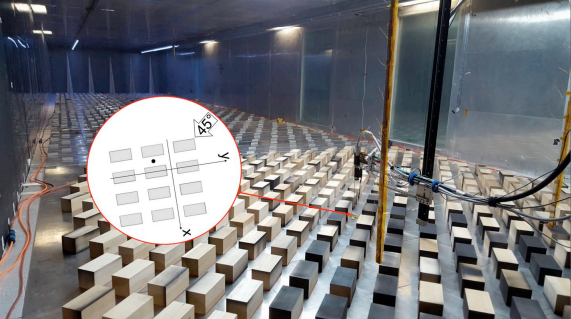
\includegraphics[scale=0.3]{imgs/sef_dataset_image.png}
%             \end{figure}
%     \end{itemize}
%     \item \textbf{NSBL - Complex Topography test cases:}
%     \begin{itemize}
%         \item from COST dataset: Cases \textit{Michelstadt} with an idealised urban geometry, and the \textit{CUTE} wind tunnel experiment with realistic representation of a European city.
%         \begin{figure}[h!]
%             \centering
%             \begin{minipage}{0.38\textwidth}
%                 \centering
%                 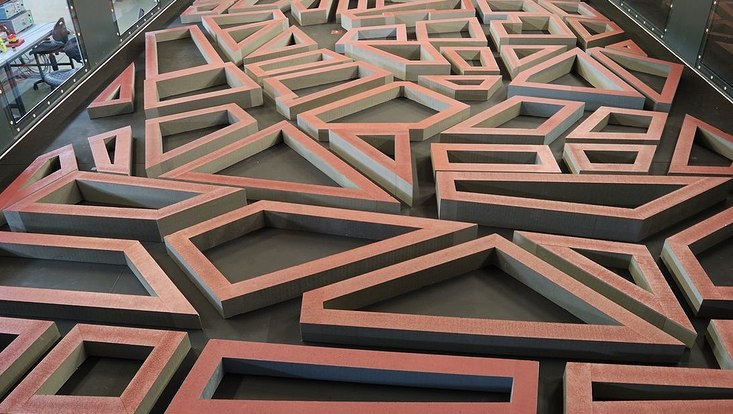
\includegraphics[width=\textwidth]{imgs/michelstad.jpg}
%                 \caption{Michelstadt wind tunnel experiment (COST-M)}
%             \end{minipage}
%             \hfill
%             \begin{minipage}{0.38\textwidth}
%                 \centering
%                 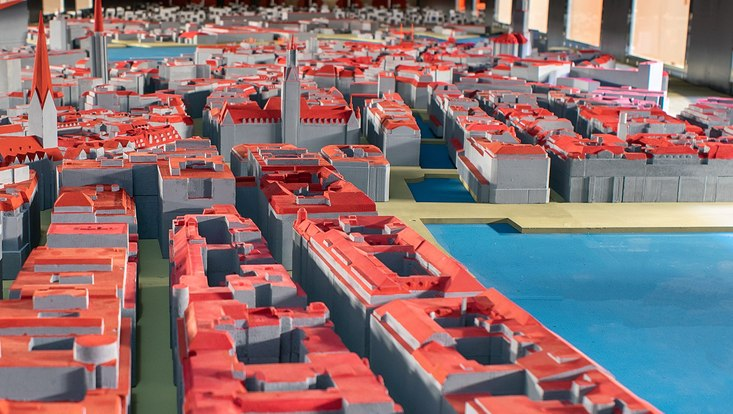
\includegraphics[width=\textwidth]{imgs/cute.jpg}
%                 \caption{CUTE wind tunnel experiment (COST-C-WT)}
%             \end{minipage}
%         \end{figure}
%     \end{itemize}
%
%     \item \textbf{SBL - Simple Obstacles test cases:}
%     \begin{itemize}
%         \item from StratEnFlo Dataset: street canyon with and without dispersion of heavy gas (SBL configuration, SEF-B).
%     \end{itemize}
%     \item \textbf{CBL - Simple Obstacles test cases:}
%     \begin{itemize}
%         \item from StratEnFlo Dataset: street canyon with and without dispersion of heavy gas (CBL configuration, SEF-C)
%         \item from TPU Dataset: single building with dispersion of neutral substance (called \textit{non-isothermal case}, TPU-B).
%         \begin{figure}[h!]
%             \centering
%             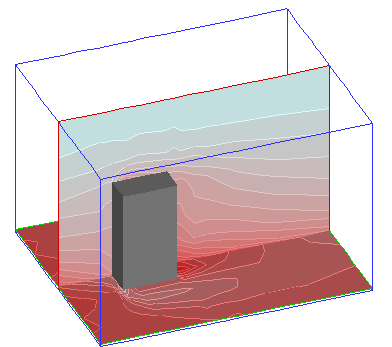
\includegraphics[width=0.4\textwidth]{imgs/tpu_2.png}
%         \end{figure}
%     \end{itemize}
%     \item \textbf{Real-world scenario test cases}
%     \begin{itemize}
%       \item COST dataset: \textit{CUTE} field experiment in a real European city (COST-C-F)
%         \begin{figure}[h!]
%             \centering
%             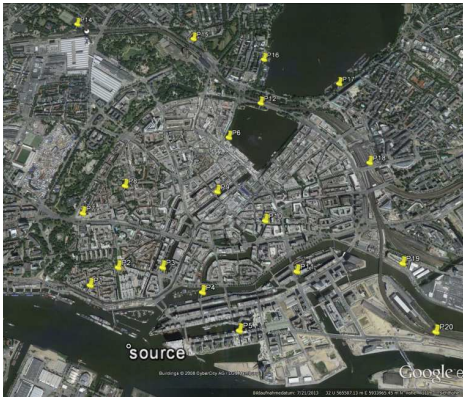
\includegraphics[width=0.4\textwidth]{imgs/cute_field_exp.png}
%             \caption{CUTE field experiment}
%         \end{figure}
%       \item TURBAN dataset: Prague field experiment (TURB-P)
%             \begin{figure}[h!]
%                 \centering
%                 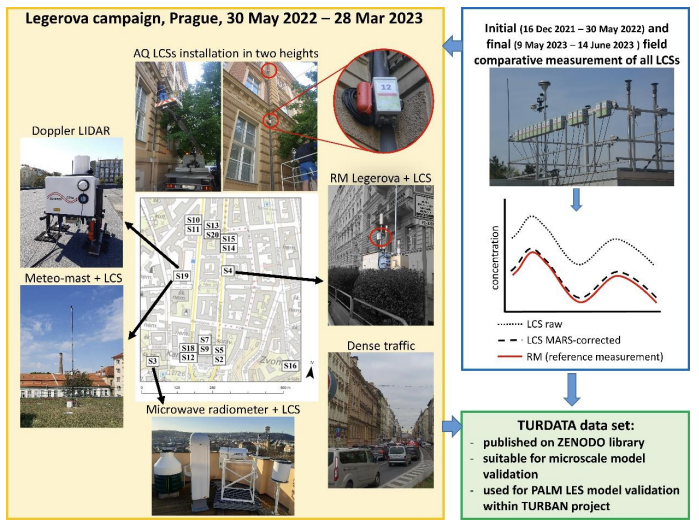
\includegraphics[width=0.4\textwidth]{imgs/turban_dataset_image.png}
%             \end{figure}
%    \end{itemize}
% \end{enumerate}
%
%

